\chapter{Introdução e Objetivos Globais}

Este relatório descreve o desenvolvimento da Proposta D, que implementa uma Modulação ASK/OOK Multiplexada na Frequência. O projeto está dividido em duas fases: o Projeto 1, que implementa o sistema em hardware estático usando Programmable Logic, e o Projeto 2, que integra o Processing System para dar controlo e configuração dinâmica ao sistema.

Os objetivos do sistema base incluem: implementar os moduladores ASK e OOK no fabric da FPGA (Pynq-Z2), aplicar a técnica de multiplexagem por divisão na frequência (FDM), controlar de forma independente o ganho de cada canal, e implementar uma secção que emula o meio físico de transmissão. Também é necessário um mecanismo de seleção dinâmica dos sinais intermédios, para simplificar a validação, encaminhando-os para a saída e para inspeção por Integrated Logic Analyzer (ILA).

A Figura \ref{fig:relatorio_diagrama_proposta_d} mostra o diagrama de blocos da arquitetura da Proposta D.

\begin{figure}[H]
    \centering
    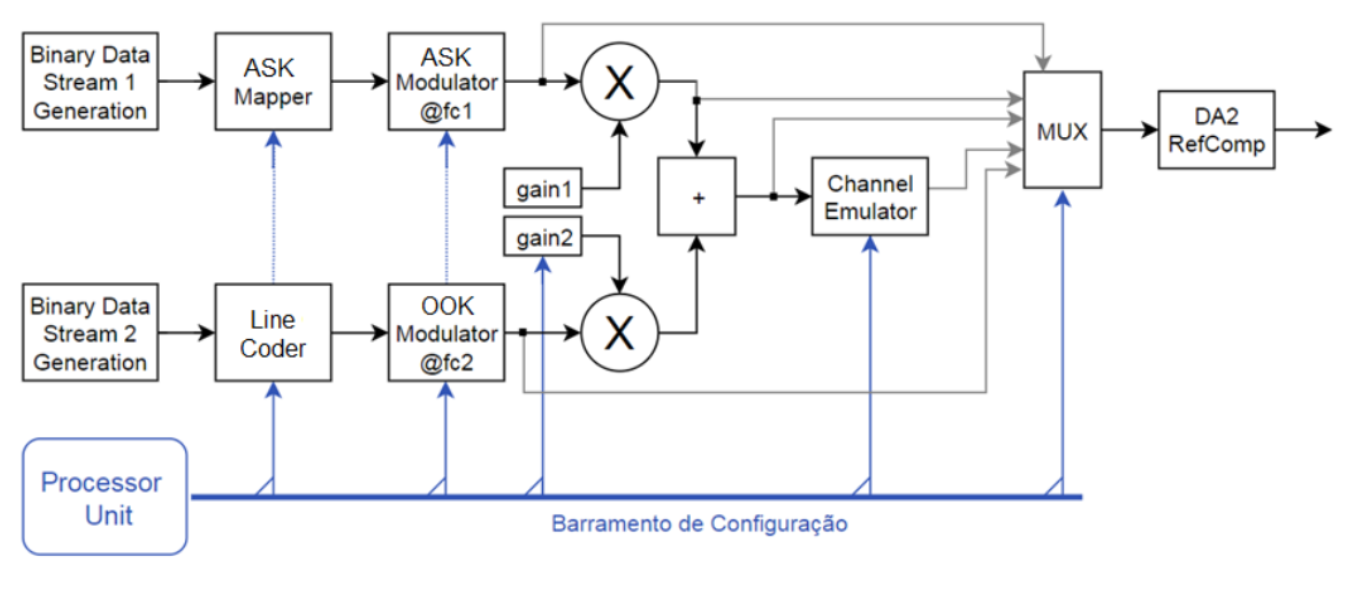
\includegraphics[width=0.8\textwidth]{imgs/relatorio_diagrama_proposta_d.png}
    \caption{Diagrama da Proposta D.}
    \label{fig:relatorio_diagrama_proposta_d}
\end{figure}
